% !TEX root = Sudoku.tex

\begin{figure}[t]
    \begin{center}
        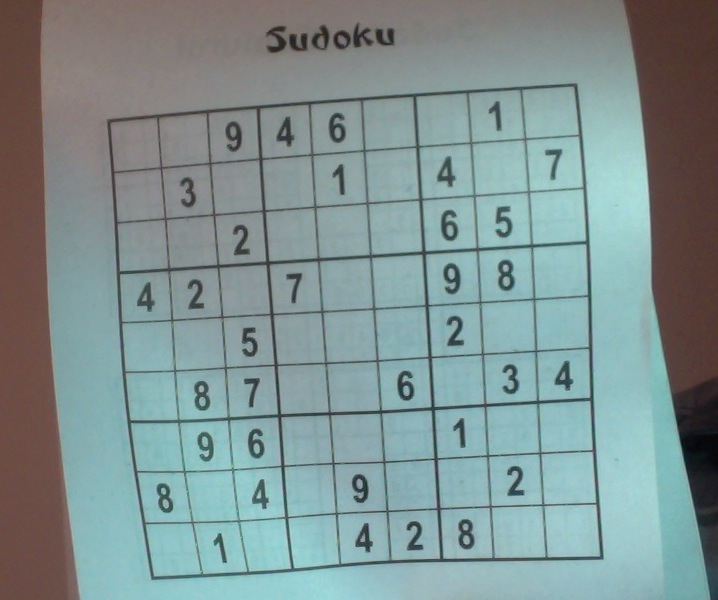
\includegraphics[width=.5\textwidth]{Abbildungen/Input}
    \end{center}
    \caption{Das verwendete Testbild}
    \label{fig:Input}
\end{figure}

\section{Methodik}
Zum Lösen dieser Aufgabe wird die Programmiersprache \emph{Python 2.7} verwendet.
Für diese steht in Form der Open-Source Library \emph{OpenCV} eine leistungsstarke Bibliothek zur Bildverarbeitung zur Verfügung.
OpenCV selbst ist in C++ geschrieben, bietet jedoch entsprechende Python-Bindings an.

Für die Erkennung der Ziffern wird die von Google entwickelte \emph{Tesseract}-Library verwendet. Auch für diese existieren Python-Bindings in Form von \emph{python-tesseract}.

Als Eingangsbild wird das Bild aus Abbildung~\ref{fig:Input} verwendet. Dieses wurde mit der Webcam eines MacBook Pro aufgenommen.

\subsection{Bild-Vorverarbeitung}
Das Bild wird zunächst in Graufstufen umgesetzt, da Farben vernachlässigt werden können.

\begin{figure}[h!]
    \begin{center}
        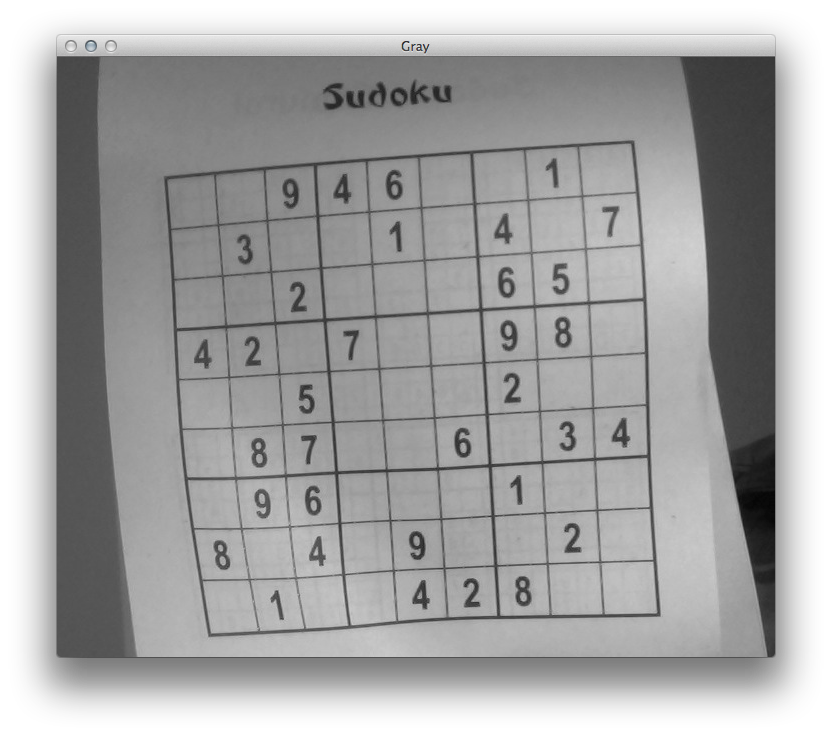
\includegraphics[width=.5\textwidth]{Abbildungen/gray}
    \end{center}
\end{figure}

Anschließend wird das Bild mit einem adaptiven Threshold binärisiert. Ein einfacher Threshold eignet sich nicht, da die Licht- und Kontrastverhältnissen unbekannt sind.

\begin{figure}[h!]
    \begin{center}
        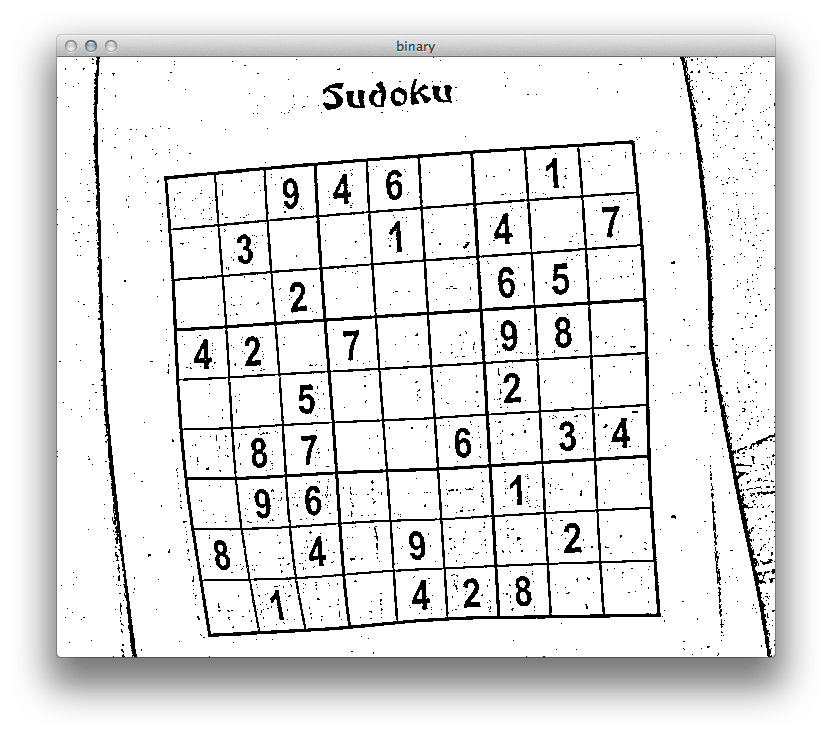
\includegraphics[width=.5\textwidth]{Abbildungen/binary}
    \end{center}
\end{figure}

Um das Rauschen zu entfernen, wird das Bild mit einem 3x3 Medianfilter gefiltert.

\begin{figure}[h!]
    \begin{center}
        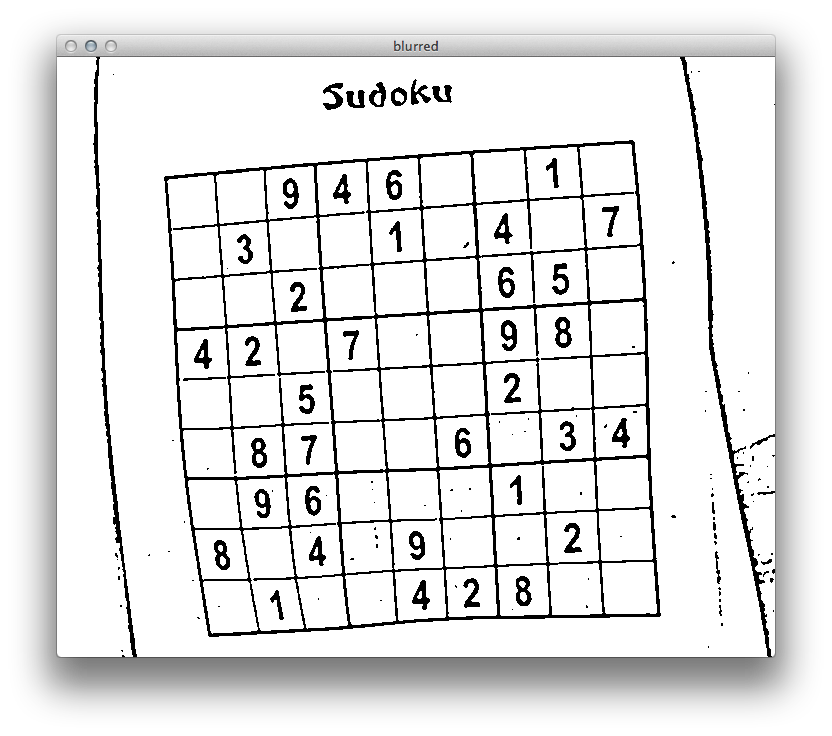
\includegraphics[width=.5\textwidth]{Abbildungen/median}
    \end{center}
\end{figure}


\subsection{Sudoku lokalisieren}
Um die Position des Sudokus zu bestimmen werden zunächst alle Konturen im Bild ermittelt. Dazu muss das binärisierte Bild invertiert werden, da der Algorithmus weiße Pixel als Objektpixel erwartet.
Alle Konturen werden über folgende Kriterien gefiltert:

\begin{enumerate}
    \item Das umschließende Rechteck muss annähernd quadratisch sein. Dazu werden die Seitenverhältnisse überprüft.
    \item Um kleine Konturen auszuschließen, wird eine Mindestfläche vorgegeben.
    \item Hinzu kommt ein Mindestwert für das Verhältnis der Konturfläche zur Fläche des umschließenden Rechtecks, um beispielsweise ``L''-förmige Konturen auszuschließen.
\end{enumerate}

Von allen Konturen, die diese Bedingungen erfüllen, wird diejenige mit der größten Konturfläche ausgewählt.


\subsection{Sudoku isolieren und transformieren}
Das umschließende Rechteck der Kontur stellt nur in Spezialfällen die tatsächliche Kontur des Sudokus dar.
Um die Eckpunkte des Sudokus im Bild zu ermitteln, wird daher die gefundene Kontur mit einem Linienzug approximiert.
Über Parameter der Funktion lässt sich der maximal gültige Fehler der Approximation einstellen.
So kann erreicht werden, dass die Approximation aus genau vier Punkten besteht, die dann die Eckpunkte darstellen.

Der zulässige Fehler ist abhängig vom Umfang der Kontur.
Er muss so eingestellt werden, dass leichte Verformungen noch zulässig sind, die Ecken aber zuverlässig erkannt werden.

Wenn die Kontur mit vier Punkten approximiert werden konnte, wird zur Separation eine Maske erstellt.
Dazu wird auf einen schwarzen Hintergrund die Kontur des Sudokus gezeichnet und weiß gefüllt.
Dieses Bild wird invertiert und mit dem bereits binärisierten Bild verodert.
Das Resultat ist das isolierte Sudoku auf weißem Hintergrund.
Dies war notwendig, da auf schwarzem Hintergrund die äußerste Feldbegrenzung verschwindet.

\begin{figure}[h!]
    \begin{center}
        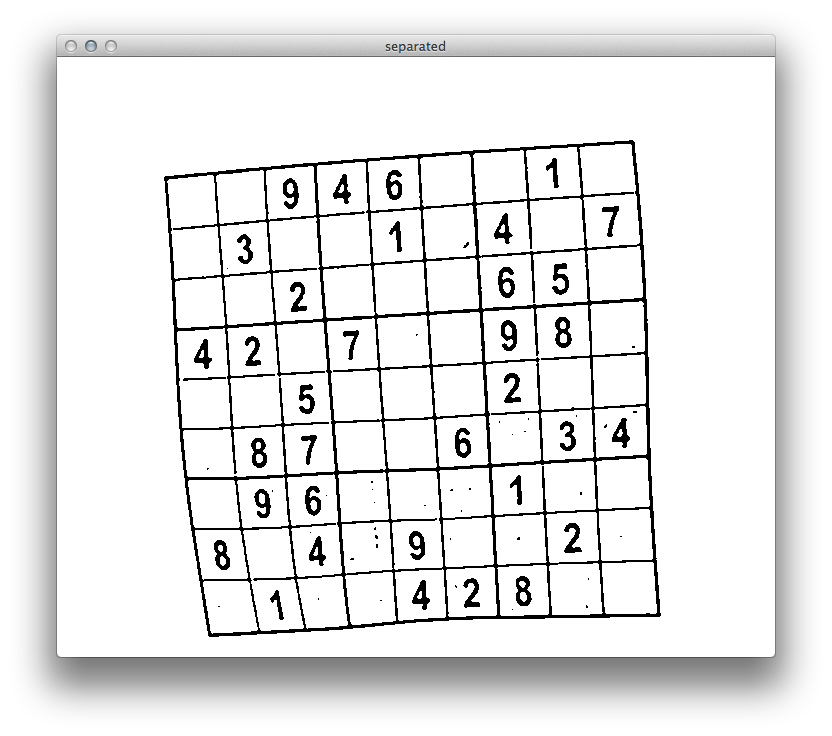
\includegraphics[width=.5\textwidth]{Abbildungen/separated}
    \end{center}
\end{figure}

Das isolierte Sudoku wird anhand der approximierten Eckpunkte perspektivisch zu einem Quadrat der Größe 450x450px transformiert.
Je nach Biegung des Papiers sind im Quadrat und an den Außenrändern noch perspektivische Verzerrungen vorhanden. Um zu verhindern, dass diese verzerrten Randbereiche abgeschnitten werden, wird ein zusätzlicher Abstand von 50px hinzugefügt.

Zuerst werden die Eckpunkte des Zielquadrats festgelegt und den approximierten Eckpunkten zugewiesen. Daraus ergibt sich die Transformationsmatrix, die anschließend auf das isolierte Sudoku angewendet wird.

\begin{figure}[h!]
    \begin{center}
        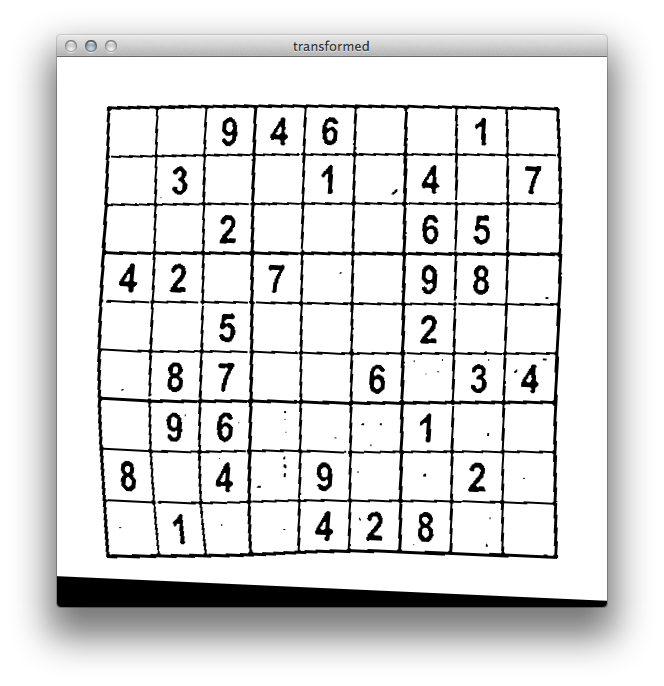
\includegraphics[width=.5\textwidth]{Abbildungen/transformed}
    \end{center}
\end{figure}


\subsection{Gitteranalyse}

